\documentclass[10pt,a4paper]{article}
\usepackage[utf8]{inputenc}
\usepackage{amsmath}
\usepackage{amsfonts}
\usepackage{amssymb}
\begin{document}
\begin{figure*}[t!]
    \centering
    \begin{subfigure}[t]{0.5\textwidth}
        \centering
        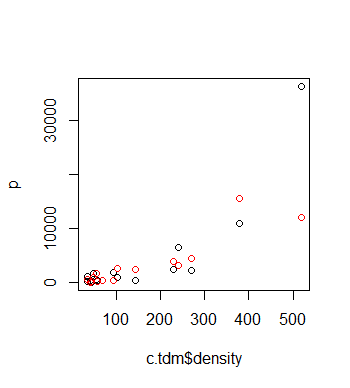
\includegraphics[height=1.2in]{pictures/Modell_1/repeat = 30/image_30-4/Rplot}
    \end{subfigure}%
    ~ 
    \begin{subfigure}[t]{0.5\textwidth}
        \centering
        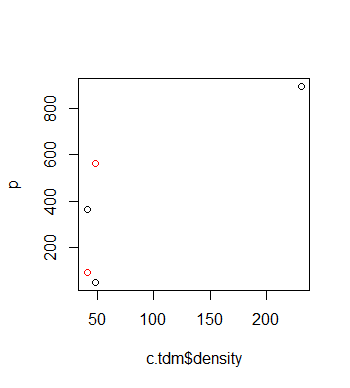
\includegraphics[height=1.2in]{pictures/Modell_1/repeat = 30/image_30-4/Rplot01}
    \end{subfigure}
\end{figure*}

\begin{figure*}[t!]
    \centering
    \begin{subfigure}[t]{0.5\textwidth}
        \centering
        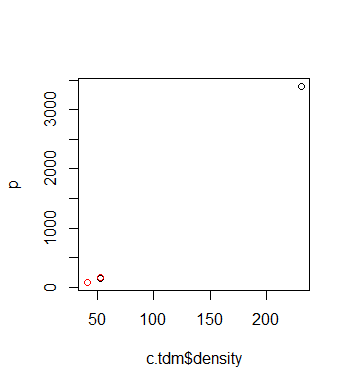
\includegraphics[height=1.2in]{pictures/Modell_1/repeat = 30/image_30-5/Rplot}
    \end{subfigure}%
    ~ 
    \begin{subfigure}[t]{0.5\textwidth}
        \centering
        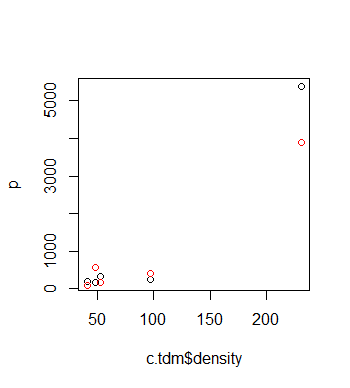
\includegraphics[height=1.2in]{pictures/Modell_1/repeat = 30/image_30-5/Rplot01}
    \end{subfigure}
\end{figure*}

\begin{figure*}[t!]
    \centering
    \begin{subfigure}[t]{0.5\textwidth}
        \centering
        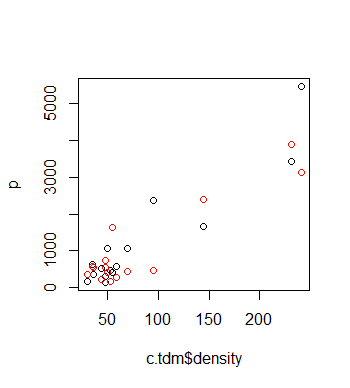
\includegraphics[height=1.2in]{pictures/Modell_1/repeat = 30/image_30-8/Rplot}
    \end{subfigure}%
    ~ 
    \begin{subfigure}[t]{0.5\textwidth}
        \centering
        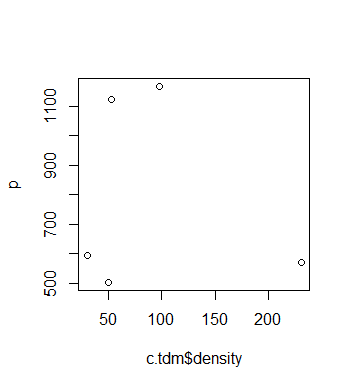
\includegraphics[height=1.2in]{pictures/Modell_1/repeat = 30/image_30-8/Rplot01}
    \end{subfigure}
\end{figure*}
\end{document}